\documentclass[tikz]{standalone}
\usetikzlibrary{mindmap}
\begin{document}
    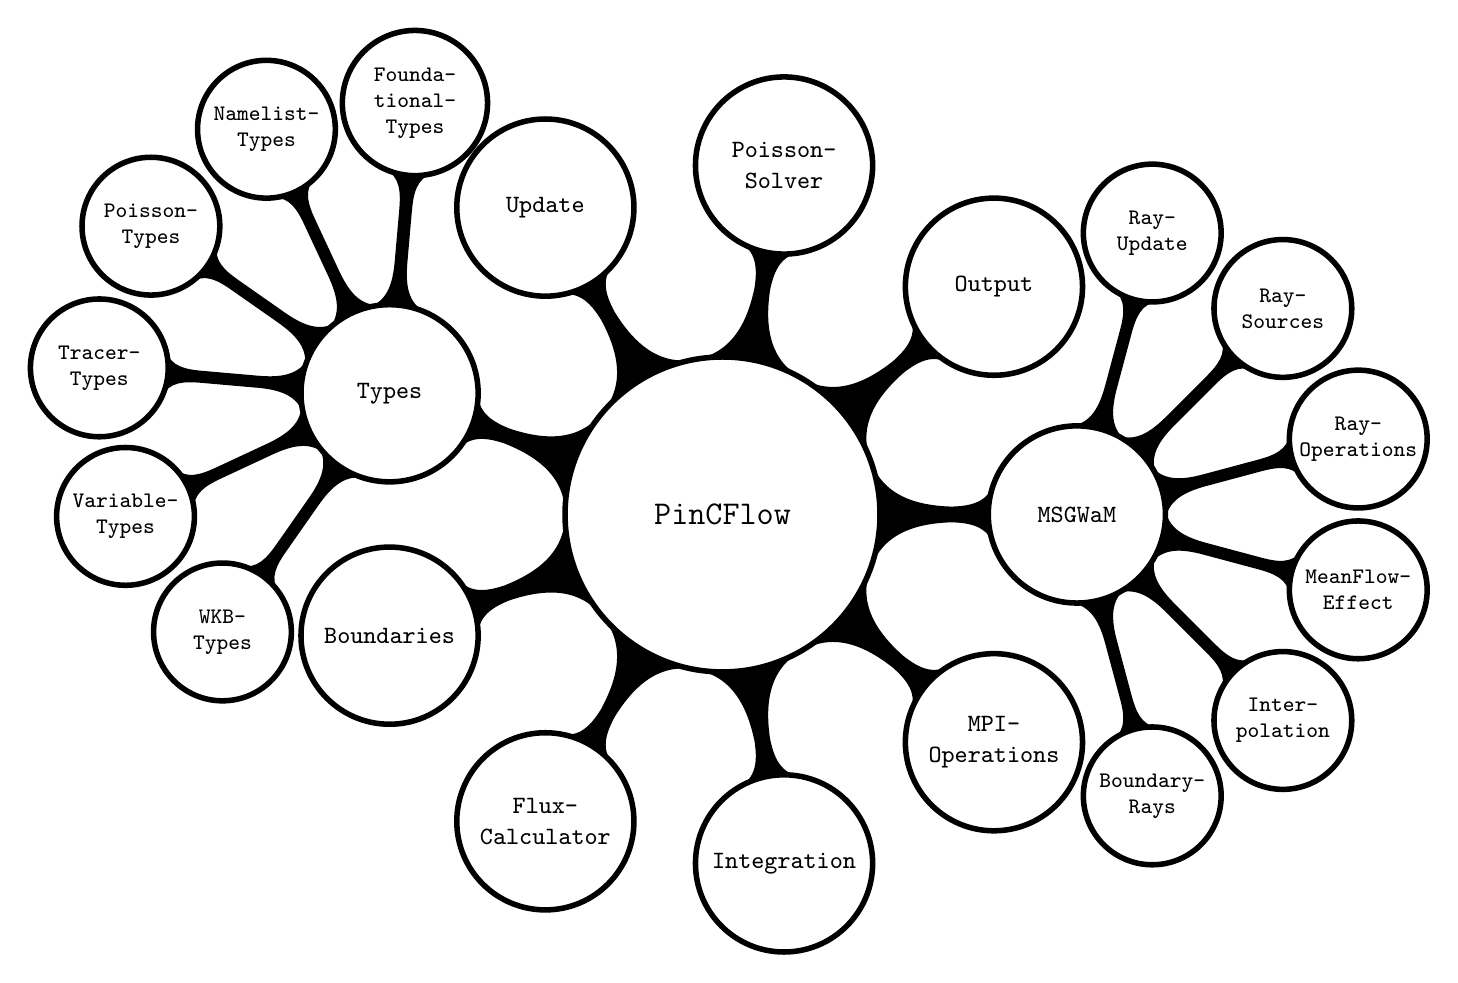
\begin{tikzpicture}[mindmap, grow cyclic, line width = 2pt, execute at begin node = \hspace{0pt}\texttt, every node/.style = {concept, fill = white}, level 1/.append style = {sibling angle = 40, level distance = 4.5cm}, level 2/.append style = {sibling angle = 30, level distance = 3.7cm}]
        \node {PinCFlow}
            child {node {Boundaries}}
            child {node {Flux-\\Calculator}}
            child {node {Integration}}
            child {node {MPI-\\Operations}}
            child {node {MSGWaM}
                child {node {Boundary-\\Rays}}
                child {node {Inter-\\polation}}
                child {node {MeanFlow-\\Effect}}
                child {node {Ray-\\Operations}}
                child {node {Ray-\\Sources}}
                child {node {Ray-\\Update}}}
            child {node {Output}}
            child {node {Poisson-\\Solver}}
            child {node {Update}}
            child {node {Types}
                child {node {Founda-\\tional-\\Types}}
                child {node {Namelist-\\Types}}
                child {node {Poisson-\\Types}}
                child {node {Tracer-\\Types}}
                child {node {Variable-\\Types}}
                child {node {WKB-\\Types}}};
    \end{tikzpicture}
\end{document}
